\chapter{概述}

本章介绍课程管理系统的项目背景、构成本文的相关基础知识并简要介绍 Model View ViewModel (MVVM) 模式、Functional Reactive Programming (FRP) 的概念及特性。

\section{项目背景与目标}

从软件行业诞生以来,办公自动化就是软件系统开发的支柱领域,随着近年来互联网的飞速发展,传统的信息自动化服务提供商在技术跟进和用户体验上都十分缓慢甚至与消费级互联网产品产生了较大的差距。企业与单位在使用传统信息自动化服务的过程当中需要耗费大量的财力、人力与时间成本对员工进行专业培训等工作,造成了极大的浪费。其中的原因在于传统的信息自动化服务注重功能的实现而缺乏用户体验设计,导致系统使用的学习曲线十分陡峭,诸多传统信息自动化服务需要依靠分发系统使用说明书向用户提供系统使用方面的支持,甚至一些更复杂的系统需要对用户进行专业培训。

面向大众消费群体的互联网产品则有着截然相反的特征,作为面向大众消费群体而设计的软件,互联网产品的设计者们必须从用户角度出发,将用户体验设计与软件功能设计放到同等重要的位置进行考量。因此,互联网产品往往拥有更加优秀的交互体验、更加平缓的学习曲线使得大多数用户能够在没有使用经验的情况下快速完成用户目标。

互联网产品从用户出发的角度来源于互联网产品行业的激烈竞争和对用户量的强烈需求,更优秀的用户体验意味着容易争取到更多的用户、在互联网产业中拥有更强的竞争力,这样的产品才能在互联网行业内生存下来。传统的信息自动化服务行业已形成一定的产业格局,竞争更多的表现在营销、资本等非产品的因素方面,因而传统的信息自动化服务在技术跟进以及用户体验上的改进都是十分缓慢的。

在 Software as a Service (SaaS) 的市场潮流下开放源代码 (Open Source) 产品正在逐渐主导软件产品的市场,最典型的开源产品如 Linux 操作系统就有多家软件公司为其提供技术支持。开源产品的更新周期往往很短,技术跟进迅速。现在,大量开源产品正支持着互联网与移动互联网产品的开发。

本项目通过吸收借鉴移动互联网的设计思路,以开放源代码的方式设计并实现课程管理系统,同时,通过课程管理系统的设计与实现,总结分析软件系统的设计方法和设计模式,探究系统架构设计的问题和解决方案。

\section{同步与异步编程模型}

同步与异步原本来自数字信号设计中的“时钟”的概念,在编程模型的角度定义“同步”为计算机程序执行的任一时刻程序仅执行一个操作,“异步”则定义为计算机程序执行的任一时刻可能有多个操作在同时执行。这里的“操作”是一个逻辑上的概念\footnote{也可以将这里的“操作”理解为“输入输出(I/O)”},比如“读取磁盘”、“等待用户输入”、“执行计算任务”。需要注意的是同步与异步仅仅在编程模型的范畴进行讨论,与并行计算这样的“实现”并没有直接的关联,使用异步编程模型设计的程序具有并行能力。

在软件产品的设计过程中同步编程模型具有很大的局限性,程序在某一时刻只能执行一个操作(如 DOS 单任务操作系统),这样的产品在与用户交互的过程中用户需要不断等待程序执行完成后再进行输入,用户体验显然是不良好的,在图形用户界面程序中如果应用同步编程模型,用户将需要在程序执行其他操作的时候(不在等待用户输入)忽略用户的所有操作。显然,在这种情况下我们需要使用异步编程模型在相应用户交互的同时处理其他的逻辑。

异步的编程模型带来一个问题——状态的维护,由于多个异步操作之间可能存在状态的共享或者相互影响,典型的例子: 用户撤销了某个正在进行中的操作,这就给命令式(Imperative)的异步编程带来了很大的难度,下节将就这一问题进行讨论。

\section{命令式与声明式编程范式}

命令式(Imperative)编程范式使用“语句”和“变量”组织一个程序,C、C++、Java 等都是常见的命令式编程语言。

命令式编程语言逐语句执行的特点可以很容易的表达同步编程模型的逻辑,大多数不需要与用户进行交互的程序都可以使用命令式语言进行简单清晰的描述。

命令式编程语言在描述异步逻辑时会遇到很大的局限性——状态的管理,命令式程序收到一个异步操作时可能进入的执行分支在最糟糕的情况下(异步逻辑高度耦合)将呈指数增长,为了解决这一问题,大量的状态管理机制被设计出来: 线程、锁、事件队列,这些机制的引入很好地解决了命令式编程语言表达异步逻辑的问题。

命令式编程语言的这种局限性在于命令式编程语言是通过语句的先后关系来确定变量(数据)的依赖关系的,而在异步(多交互)条件下需要在一定程度上清除大量由“语句先后”产生的无效的数据依赖,比如“用户输入”是不依赖“数据下载”操作的,而命令式编程中“读取用户输入”语句出现在了“数据下载”语句之前则产生了一个“语句先后依赖“,异步编程模型下这两个逻辑都只依赖”异步操作“因此命令式语言中需要将两者间“语句先后依赖“的隐含语义给予消除才能使程序形成正确的依赖关系。

与命令式编程语言不同,声明式编程范式通过描述数据关系”定义“程序的目标将命令式编程中的计算步骤转换为一种”推导“过程。声明式编程范式的性质表现为在声明程序的过程中显示指定了所有数据依赖,而不存在命令式语言中会隐式出现的”语句先后依赖“,这样的结构使声明式语言非常适合于描述异步逻辑。但声明式语言在描述同步逻辑时将比命令式语言的表述更加复杂甚至晦涩,因此,Haskell 这样的通用函数式语言中设计了 $do$ 块让编译器进行 Continuation-Passing Style (CPS) 变换\footnote{Wikipedia: Continuation-Passing Style} 以实现对”逐语句“行为的模拟。

相对的,为了让命令式编程语言能够使用”逐语句“的方法定义异步过程,Python 这样的通用命令式语言中设计了 $Generator$ 让编译器进行逆 CPS 变换以实现对隐含的“语句先后依赖“关系的解除,不同的是 CPS 变换不依赖作用域而逆 CPS 变换将依赖一个代码域以映射 $Continuation$。

\section{Model~View~Controller~架构模式}

MVC 架构模式是由 Trygve Reenskaug 在 1978 年提出\cite{reenskaug1979thing} 用于实现图形用户界面的一种设计模式,最初实现于 Smalltalk 语言平台。

\begin{figure}[!h]
\begin{center}
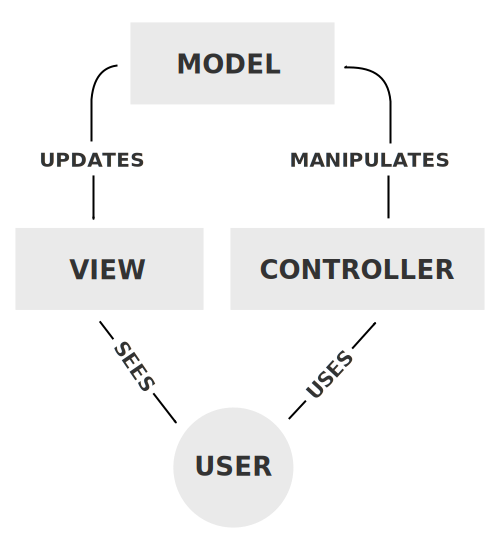
\includegraphics[scale=0.5]{figures/pattern-mvc.pdf}
\caption{MVC 架构典型交互示意图\label{MVCOverview}}
\end{center}
\end{figure}

典型的 MVC 模式(如图~\ref{MVCOverview})将系统分成 Model(模型)、View(视图)、Controller(控制器) 三个部分: Model 对象用于处理数据和业务操作、View 对象控制视图逻辑、Controller 负责处理用户操作。MVC 架构作为许多互联网产品和应用的基础架构在各大开发平台都有成熟的解决方案和技术框架\footnote{如 Ruby-on-Rails、ThinkMVC 等广泛应用的 Web 框架都基于 MVC 架构进行开发}。

可以看到 MVC 模式仅仅使用 Model、View、Controller 对系统进行了划分,而 MVVM 模式正是对 Controller 进行了详细设计。

\section{Model~View~ViewModel~架构模式}

用户交互(User Interaction)在消费级产品开发中的地位近年来正不断提升,交互设计和实现正成为产品开发中最重要也最复杂的环节之一。随着互联网的发展、富交互应用(Rich Interaction Application, RIA)的兴起,交互设计正走向越来越复杂的方向。使用传统的命令式编程(Imperative Programming)实现用户交互逻辑的局限性也不断显现出来。

Microsoft 在 Windows Presentation Framework (WPF) 中引入的 Model View ViewModel (MVVM) 模式近年来得到了相当广泛的关注和应用。MVVM模式作为如今最成功的图形用户界面(Graphical User Interface, GUI)开发模式之一,使用面向对象的方法实现了”声明式“的界面逻辑定义方法,解决了命令式编程方法在处理异步逻辑时难于维持代码逻辑连续性的问题。

\begin{figure}[!h]
\begin{center}
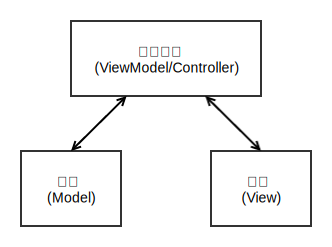
\includegraphics[scale=0.7]{figures/pattern-mvvm.pdf}
\caption{MVVM 架构典型交互示意图\label{MVVMOverview}}
\end{center}
\end{figure}

Model~View~ViewModel (MVVM) 模式是 Model~View~Controller (MVC) 模式的一种特例(见图~\ref{MVVMOverview}): MVC 模式中 Controller 负责进行的界面业务逻辑部分抽象为 ViewModel 以及 Binder 组合。一方面利用 ViewModel 管理交互状态、另一方面通过 Binder 将状态通过 View 进行展示。用户产生的交互事件也经由 Binder 传递至 ViewModel 对用户界面的状态以及 Model 状态产生影响。

MVVM 模式的一大设计亮点在于“ViewModel 继承于 Model” 即: ViewModel 可以将另一个 ViewModel 实例作为 Model 进行数据请求。这是 ViewModel 与 Controller 之间最大的不同,也是 ViewModel 较 Controller 实现拥有更高的可复用性以及更良好的可测试性的原因。

另外,MVVM 模式解除了 Controller 代码与视图实现之间的耦合关系,界面设计人员仅需要在XAML(对WPF的情况)文档中描述视图对象所需要绑定(bind)的数据位置(属性名称)即可完成用户交互设计任务,而在 MVC 模式中设计者需要书写 Controller 代码以描述视图对象所需要的呈现数据。

MVVM 模式在普遍用于用户交互开发的 JavaScript 语言中也得到了类似的实现,如 AngularJS、KnockoutJS 等开发框架。

课程管理系统作为面向业务产品的典型代表,工程规模足够体现设计模式的各项性能。本文以课程管理产品的设计与开发为例,尝试解释 MVVM 设计模式的设计方法。

\section{Functional Reactive Programming}

Functional Reactive Programming (FRP) 是使用声明式 (Declarative) 方法描述系统行为的编程方法。FRP 的主要思想是将系统抽象为行为(Behaviors)和事件(Events),使用行为表示系统中随时域连续变化的值、事件表示一系列按一定时序触发的离散值\cite{Wan:2000:FRP:358438.349331}。最初,FRP 方法被应用于 Haskell 的 Functional Reactive Animation (Fran) 的核心实现\cite{Elliott:1997:FRA:258949.258973}。后来,FRP 方法被广泛的用于计算机视觉、机器人以及其他控制系统的设计和实现。

简而言之,FRP 抽象系统为用户与函数(Behavior)的交互,用户事件作为函数的自变量,而模型/用户视图作为函数作用的因变量。

随着 FRP 理论的成熟与富交互应用的发展,FRP 的影响也逐渐延伸到应用开发的前沿领域,出现了许多成熟的 FRP 开发框架,如 Objective C 平台下的 ReactiveCocoa,.NET Framework 下的 ReactiveUI 以及 JavaScript 平台下的 Reactive.js 等\footnote{虽然这些框架是实现在命令式语言平台的 Reactive Programming 框架,这里还是沿用 Haskell 中 FRP 的名称}。

FRP 方法与 MVVM 使用的 Observer 模式具有很高的相似性,本文将在后面的章节围绕此问题进行一番讨论并提出作者对 MVVM 架构模式的理解,在此基础上使用 Monad 高阶函数\cite{raey}开发 MVVM 框架并测试该框架在课程管理系统中实际进行富交互应用开发的性能。

后文分成五个部分: 第二章、第三章分别介绍系统的需求分析和概要设计,第四章引入有关 MVVM 模式与 Reactive Programming 的讨论、描述 ReactiveVM 的设计思路,第五章讨论实现过程中出现的探索性过程,第六章对项目的开发过程进行一个总结并描述一下对未来研究方向的展望。

